% Options for packages loaded elsewhere
\PassOptionsToPackage{unicode}{hyperref}
\PassOptionsToPackage{hyphens}{url}
%
\documentclass[
]{article}
\usepackage{amsmath,amssymb}
\usepackage{lmodern}
\usepackage{iftex}
\ifPDFTeX
  \usepackage[T1]{fontenc}
  \usepackage[utf8]{inputenc}
  \usepackage{textcomp} % provide euro and other symbols
\else % if luatex or xetex
  \usepackage{unicode-math}
  \defaultfontfeatures{Scale=MatchLowercase}
  \defaultfontfeatures[\rmfamily]{Ligatures=TeX,Scale=1}
\fi
% Use upquote if available, for straight quotes in verbatim environments
\IfFileExists{upquote.sty}{\usepackage{upquote}}{}
\IfFileExists{microtype.sty}{% use microtype if available
  \usepackage[]{microtype}
  \UseMicrotypeSet[protrusion]{basicmath} % disable protrusion for tt fonts
}{}
\makeatletter
\@ifundefined{KOMAClassName}{% if non-KOMA class
  \IfFileExists{parskip.sty}{%
    \usepackage{parskip}
  }{% else
    \setlength{\parindent}{0pt}
    \setlength{\parskip}{6pt plus 2pt minus 1pt}}
}{% if KOMA class
  \KOMAoptions{parskip=half}}
\makeatother
\usepackage{xcolor}
\usepackage[margin=1in]{geometry}
\usepackage{color}
\usepackage{fancyvrb}
\newcommand{\VerbBar}{|}
\newcommand{\VERB}{\Verb[commandchars=\\\{\}]}
\DefineVerbatimEnvironment{Highlighting}{Verbatim}{commandchars=\\\{\}}
% Add ',fontsize=\small' for more characters per line
\usepackage{framed}
\definecolor{shadecolor}{RGB}{248,248,248}
\newenvironment{Shaded}{\begin{snugshade}}{\end{snugshade}}
\newcommand{\AlertTok}[1]{\textcolor[rgb]{0.94,0.16,0.16}{#1}}
\newcommand{\AnnotationTok}[1]{\textcolor[rgb]{0.56,0.35,0.01}{\textbf{\textit{#1}}}}
\newcommand{\AttributeTok}[1]{\textcolor[rgb]{0.77,0.63,0.00}{#1}}
\newcommand{\BaseNTok}[1]{\textcolor[rgb]{0.00,0.00,0.81}{#1}}
\newcommand{\BuiltInTok}[1]{#1}
\newcommand{\CharTok}[1]{\textcolor[rgb]{0.31,0.60,0.02}{#1}}
\newcommand{\CommentTok}[1]{\textcolor[rgb]{0.56,0.35,0.01}{\textit{#1}}}
\newcommand{\CommentVarTok}[1]{\textcolor[rgb]{0.56,0.35,0.01}{\textbf{\textit{#1}}}}
\newcommand{\ConstantTok}[1]{\textcolor[rgb]{0.00,0.00,0.00}{#1}}
\newcommand{\ControlFlowTok}[1]{\textcolor[rgb]{0.13,0.29,0.53}{\textbf{#1}}}
\newcommand{\DataTypeTok}[1]{\textcolor[rgb]{0.13,0.29,0.53}{#1}}
\newcommand{\DecValTok}[1]{\textcolor[rgb]{0.00,0.00,0.81}{#1}}
\newcommand{\DocumentationTok}[1]{\textcolor[rgb]{0.56,0.35,0.01}{\textbf{\textit{#1}}}}
\newcommand{\ErrorTok}[1]{\textcolor[rgb]{0.64,0.00,0.00}{\textbf{#1}}}
\newcommand{\ExtensionTok}[1]{#1}
\newcommand{\FloatTok}[1]{\textcolor[rgb]{0.00,0.00,0.81}{#1}}
\newcommand{\FunctionTok}[1]{\textcolor[rgb]{0.00,0.00,0.00}{#1}}
\newcommand{\ImportTok}[1]{#1}
\newcommand{\InformationTok}[1]{\textcolor[rgb]{0.56,0.35,0.01}{\textbf{\textit{#1}}}}
\newcommand{\KeywordTok}[1]{\textcolor[rgb]{0.13,0.29,0.53}{\textbf{#1}}}
\newcommand{\NormalTok}[1]{#1}
\newcommand{\OperatorTok}[1]{\textcolor[rgb]{0.81,0.36,0.00}{\textbf{#1}}}
\newcommand{\OtherTok}[1]{\textcolor[rgb]{0.56,0.35,0.01}{#1}}
\newcommand{\PreprocessorTok}[1]{\textcolor[rgb]{0.56,0.35,0.01}{\textit{#1}}}
\newcommand{\RegionMarkerTok}[1]{#1}
\newcommand{\SpecialCharTok}[1]{\textcolor[rgb]{0.00,0.00,0.00}{#1}}
\newcommand{\SpecialStringTok}[1]{\textcolor[rgb]{0.31,0.60,0.02}{#1}}
\newcommand{\StringTok}[1]{\textcolor[rgb]{0.31,0.60,0.02}{#1}}
\newcommand{\VariableTok}[1]{\textcolor[rgb]{0.00,0.00,0.00}{#1}}
\newcommand{\VerbatimStringTok}[1]{\textcolor[rgb]{0.31,0.60,0.02}{#1}}
\newcommand{\WarningTok}[1]{\textcolor[rgb]{0.56,0.35,0.01}{\textbf{\textit{#1}}}}
\usepackage{graphicx}
\makeatletter
\def\maxwidth{\ifdim\Gin@nat@width>\linewidth\linewidth\else\Gin@nat@width\fi}
\def\maxheight{\ifdim\Gin@nat@height>\textheight\textheight\else\Gin@nat@height\fi}
\makeatother
% Scale images if necessary, so that they will not overflow the page
% margins by default, and it is still possible to overwrite the defaults
% using explicit options in \includegraphics[width, height, ...]{}
\setkeys{Gin}{width=\maxwidth,height=\maxheight,keepaspectratio}
% Set default figure placement to htbp
\makeatletter
\def\fps@figure{htbp}
\makeatother
\setlength{\emergencystretch}{3em} % prevent overfull lines
\providecommand{\tightlist}{%
  \setlength{\itemsep}{0pt}\setlength{\parskip}{0pt}}
\setcounter{secnumdepth}{-\maxdimen} % remove section numbering
\ifLuaTeX
  \usepackage{selnolig}  % disable illegal ligatures
\fi
\IfFileExists{bookmark.sty}{\usepackage{bookmark}}{\usepackage{hyperref}}
\IfFileExists{xurl.sty}{\usepackage{xurl}}{} % add URL line breaks if available
\urlstyle{same} % disable monospaced font for URLs
\hypersetup{
  pdftitle={Merge LA refinery data ses},
  pdfauthor={Jerry Wu},
  hidelinks,
  pdfcreator={LaTeX via pandoc}}

\title{Merge LA refinery data ses}
\author{Jerry Wu}
\date{5/1/2023}

\begin{document}
\maketitle

\begin{Shaded}
\begin{Highlighting}[]
\CommentTok{\# load data sets}
\NormalTok{full\_data }\OtherTok{\textless{}{-}} \FunctionTok{tibble}\NormalTok{()}
\NormalTok{names }\OtherTok{\textless{}{-}} \FunctionTok{c}\NormalTok{(}\AttributeTok{ws =} \StringTok{\textquotesingle{}windSpeed\textquotesingle{}}\NormalTok{, }\AttributeTok{wd =} \StringTok{\textquotesingle{}windDirection\textquotesingle{}}\NormalTok{, }\AttributeTok{H2S =} \StringTok{\textquotesingle{}Value\textquotesingle{}}\NormalTok{)}
\ControlFlowTok{for}\NormalTok{ (file }\ControlFlowTok{in} \FunctionTok{list.files}\NormalTok{(}\StringTok{\textquotesingle{}data/raw\_csv\textquotesingle{}}\NormalTok{))\{}
\NormalTok{  new\_data }\OtherTok{\textless{}{-}} \FunctionTok{read.csv}\NormalTok{(}\FunctionTok{paste0}\NormalTok{(}\StringTok{\textquotesingle{}data/raw\_csv/\textquotesingle{}}\NormalTok{, file)) }\SpecialCharTok{\%\textgreater{}\%} \FunctionTok{rename}\NormalTok{(}\FunctionTok{any\_of}\NormalTok{(names))}
  \FunctionTok{print}\NormalTok{(}\FunctionTok{sum}\NormalTok{(}\FunctionTok{is.na}\NormalTok{(new\_data}\SpecialCharTok{$}\NormalTok{H2S)))}
\NormalTok{  full\_data }\OtherTok{\textless{}{-}} \FunctionTok{bind\_rows}\NormalTok{(full\_data, new\_data)}
\NormalTok{\}}
\end{Highlighting}
\end{Shaded}

\begin{verbatim}
## [1] 0
## [1] 0
## [1] 21079
## [1] 22460
## [1] 39137
## [1] 24914
## [1] 19875
## [1] 20540
## [1] 8137
## [1] 20690
## [1] 0
## [1] 34281
## [1] 0
\end{verbatim}

\begin{Shaded}
\begin{Highlighting}[]
\NormalTok{full\_data }\OtherTok{\textless{}{-}}\NormalTok{ full\_data }\SpecialCharTok{\%\textgreater{}\%} \FunctionTok{mutate}\NormalTok{(}\AttributeTok{DateTime =} \FunctionTok{as.POSIXct}\NormalTok{(DateTime, }\AttributeTok{format=}\StringTok{"\%m/\%d/\%Y \%H:\%M"}\NormalTok{, }\AttributeTok{tz =} \StringTok{\textquotesingle{}UTC\textquotesingle{}}\NormalTok{),}
                                  \AttributeTok{Date.Time =} \FunctionTok{as.POSIXct}\NormalTok{(Date.Time, }\AttributeTok{format=}\StringTok{"\%m/\%d/\%Y \%H:\%M"}\NormalTok{, }\AttributeTok{tz =} \StringTok{\textquotesingle{}UTC\textquotesingle{}}\NormalTok{),}
                                  \AttributeTok{Date.Time.First =} \FunctionTok{as.POSIXct}\NormalTok{(Date.Time.First, }\AttributeTok{format=}\StringTok{"\%m/\%d/\%Y \%H:\%M"}\NormalTok{, }\AttributeTok{tz =} \StringTok{\textquotesingle{}UTC\textquotesingle{}}\NormalTok{))}
\NormalTok{full\_data }\OtherTok{\textless{}{-}}\NormalTok{ full\_data }\SpecialCharTok{\%\textgreater{}\%} 
  \FunctionTok{mutate}\NormalTok{(}\AttributeTok{day =} \FunctionTok{format}\NormalTok{(DateTime, }\StringTok{"\%Y{-}\%m{-}\%d"}\NormalTok{)) }\SpecialCharTok{\%\textgreater{}\%}
  \FunctionTok{mutate}\NormalTok{(}\AttributeTok{day =} \FunctionTok{if\_else}\NormalTok{(}\FunctionTok{is.na}\NormalTok{(day), }\FunctionTok{format}\NormalTok{(Date.Time, }\StringTok{"\%Y{-}\%m{-}\%d"}\NormalTok{), day)) }\SpecialCharTok{\%\textgreater{}\%}
  \FunctionTok{mutate}\NormalTok{(}\AttributeTok{day =} \FunctionTok{if\_else}\NormalTok{(}\FunctionTok{is.na}\NormalTok{(day), }\FunctionTok{format}\NormalTok{(Date.Time.First, }\StringTok{"\%Y{-}\%m{-}\%d"}\NormalTok{), day)) }\SpecialCharTok{\%\textgreater{}\%}
  \FunctionTok{mutate}\NormalTok{(}\AttributeTok{day =} \FunctionTok{as.POSIXct}\NormalTok{(day, }\AttributeTok{format=}\StringTok{"\%Y{-}\%m{-}\%d"}\NormalTok{)) }\SpecialCharTok{\%\textgreater{}\%}
  \FunctionTok{mutate}\NormalTok{(}\AttributeTok{yearmonth =} \FunctionTok{format}\NormalTok{(day, }\StringTok{"\%Y{-}\%m"}\NormalTok{)) }\SpecialCharTok{\%\textgreater{}\%}
  \FunctionTok{mutate}\NormalTok{(}\AttributeTok{year =} \FunctionTok{format}\NormalTok{(day, }\StringTok{"\%Y"}\NormalTok{)) }\SpecialCharTok{\%\textgreater{}\%}
  \FunctionTok{mutate}\NormalTok{(}\AttributeTok{month =} \FunctionTok{format}\NormalTok{(day, }\StringTok{"\%m"}\NormalTok{))}
\end{Highlighting}
\end{Shaded}

\begin{Shaded}
\begin{Highlighting}[]
\FunctionTok{glimpse}\NormalTok{(full\_data)}
\end{Highlighting}
\end{Shaded}

\begin{verbatim}
## Rows: 3,654,646
## Columns: 24
## $ DateTime             <dttm> 2021-10-22 15:15:00, 2021-10-22 15:20:00, 2021-1~
## $ Date.Time            <dttm> 2021-10-22 15:15:00, 2021-10-22 15:20:00, 2021-1~
## $ H2S                  <dbl> 138.79, 183.26, 149.24, 263.18, 308.97, 169.06, 2~
## $ Averaging.Hour       <chr> "5 Min", "5 Min", "5 Min", "5 Min", "5 Min", "5 M~
## $ ws                   <dbl> 7.01, 6.32, 6.73, 6.54, 8.02, 7.82, 6.99, 6.71, 6~
## $ wd                   <dbl> 276.87, 250.15, 263.97, 280.36, 269.26, 256.21, 2~
## $ latitude             <dbl> 33.83678, 33.83678, 33.83678, 33.83678, 33.83678,~
## $ longitude            <dbl> -118.2586, -118.2586, -118.2586, -118.2586, -118.~
## $ Monitor              <chr> "213th&Chico", "213th&Chico", "213th&Chico", "213~
## $ Join_Count           <int> 1, 1, 1, 1, 1, 1, 1, 1, 1, 1, 1, 1, 1, 1, 1, 1, 1~
## $ MinDist              <dbl> 2873.053, 2873.053, 2873.053, 2873.053, 2873.053,~
## $ Converted_Angle      <int> 306, 306, 306, 306, 306, 306, 306, 306, 306, 306,~
## $ Refinery             <chr> "Marathon (Carson)", "Marathon (Carson)", "Marath~
## $ Unit                 <chr> NA, NA, NA, NA, NA, NA, NA, NA, NA, NA, NA, NA, N~
## $ Date.Time.First      <dttm> NA, NA, NA, NA, NA, NA, NA, NA, NA, NA, NA, NA, ~
## $ Averaging.Hour.First <chr> NA, NA, NA, NA, NA, NA, NA, NA, NA, NA, NA, NA, N~
## $ Monitor.1            <chr> NA, NA, NA, NA, NA, NA, NA, NA, NA, NA, NA, NA, N~
## $ siteName             <chr> NA, NA, NA, NA, NA, NA, NA, NA, NA, NA, NA, NA, N~
## $ Wind_latitude        <dbl> NA, NA, NA, NA, NA, NA, NA, NA, NA, NA, NA, NA, N~
## $ Wind_longitude       <dbl> NA, NA, NA, NA, NA, NA, NA, NA, NA, NA, NA, NA, N~
## $ day                  <dttm> 2021-10-22, 2021-10-22, 2021-10-22, 2021-10-22, ~
## $ yearmonth            <chr> "2021-10", "2021-10", "2021-10", "2021-10", "2021~
## $ year                 <chr> "2021", "2021", "2021", "2021", "2021", "2021", "~
## $ month                <chr> "10", "10", "10", "10", "10", "10", "10", "10", "~
\end{verbatim}

\begin{Shaded}
\begin{Highlighting}[]
\FunctionTok{summary}\NormalTok{(full\_data)}
\end{Highlighting}
\end{Shaded}

\begin{verbatim}
##     DateTime                       Date.Time                     
##  Min.   :2019-12-17 15:35:00.0   Min.   :2019-12-17 15:35:00.00  
##  1st Qu.:2021-01-07 01:20:00.0   1st Qu.:2020-12-29 17:35:00.00  
##  Median :2021-10-11 17:25:00.0   Median :2021-10-01 14:50:00.00  
##  Mean   :2021-09-07 09:01:10.2   Mean   :2021-08-21 17:30:20.85  
##  3rd Qu.:2022-05-19 15:50:00.0   3rd Qu.:2022-04-23 21:40:00.00  
##  Max.   :2023-02-13 07:55:00.0   Max.   :2022-12-31 23:55:00.00  
##  NA's   :721231                  NA's   :1217186                 
##       H2S          Averaging.Hour           ws                wd         
##  Min.   :   0.00   Length:3654646     Min.   : 0.0      Min.   :  0.0    
##  1st Qu.:   0.24   Class :character   1st Qu.: 1.4      1st Qu.:137.8    
##  Median :   0.60   Mode  :character   Median : 2.9      Median :247.9    
##  Mean   :   1.06                      Mean   : 3.5      Mean   :211.9    
##  3rd Qu.:   1.10                      3rd Qu.: 5.0      3rd Qu.:294.0    
##  Max.   :3817.24                      Max.   :57.8      Max.   :360.0    
##  NA's   :211113                       NA's   :1153462   NA's   :1475504  
##     latitude        longitude        Monitor            Join_Count   
##  Min.   :33.78    Min.   :-118.4   Length:3654646     Min.   :1.000  
##  1st Qu.:33.79    1st Qu.:-118.4   Class :character   1st Qu.:1.000  
##  Median :33.82    Median :-118.3   Mode  :character   Median :1.000  
##  Mean   :33.83    Mean   :-118.3                      Mean   :1.949  
##  3rd Qu.:33.87    3rd Qu.:-118.3                      3rd Qu.:3.000  
##  Max.   :33.92    Max.   :-118.2                      Max.   :5.000  
##  NA's   :211113   NA's   :211113                                     
##     MinDist       Converted_Angle   Refinery             Unit          
##  Min.   : 758.7   Min.   : 11.0   Length:3654646     Length:3654646    
##  1st Qu.:1308.3   1st Qu.:189.0   Class :character   Class :character  
##  Median :1988.2   Median :209.0   Mode  :character   Mode  :character  
##  Mean   :1909.0   Mean   :198.5                                        
##  3rd Qu.:2541.9   3rd Qu.:263.0                                        
##  Max.   :3592.8   Max.   :338.0                                        
##                                                                        
##  Date.Time.First                  Averaging.Hour.First  Monitor.1        
##  Min.   :2020-03-04 14:30:00.00   Length:3654646       Length:3654646    
##  1st Qu.:2020-11-21 07:31:15.00   Class :character     Class :character  
##  Median :2021-08-05 13:07:30.00   Mode  :character     Mode  :character  
##  Mean   :2021-08-03 22:26:59.01                                          
##  3rd Qu.:2022-04-17 10:53:45.00                                          
##  Max.   :2022-12-31 23:55:00.00                                          
##  NA's   :3368232                                                         
##    siteName         Wind_latitude     Wind_longitude   
##  Length:3654646     Min.   :34        Min.   :-118     
##  Class :character   1st Qu.:34        1st Qu.:-118     
##  Mode  :character   Median :34        Median :-118     
##                     Mean   :34        Mean   :-118     
##                     3rd Qu.:34        3rd Qu.:-118     
##                     Max.   :34        Max.   :-118     
##                     NA's   :3420724   NA's   :3420724  
##       day                          yearmonth             year          
##  Min.   :2019-12-17 00:00:00.00   Length:3654646     Length:3654646    
##  1st Qu.:2021-01-07 00:00:00.00   Class :character   Class :character  
##  Median :2021-10-11 00:00:00.00   Mode  :character   Mode  :character  
##  Mean   :2021-09-06 20:10:40.56                                        
##  3rd Qu.:2022-05-19 00:00:00.00                                        
##  Max.   :2023-02-13 00:00:00.00                                        
##  NA's   :719791                                                        
##     month          
##  Length:3654646    
##  Class :character  
##  Mode  :character  
##                    
##                    
##                    
## 
\end{verbatim}

Some concerns for the data include: For TorranceAir\_H2SWind, there are
actually three sites, but only one site contains ws/wd information
What's the difference between DateTime and Date/Time? What's the
difference between Date/Time and Date/Time.First? The latter is present
in FirstMethodist

\hypertarget{compute-daily-max-h2s}{%
\section{Compute Daily Max H2S}\label{compute-daily-max-h2s}}

\begin{Shaded}
\begin{Highlighting}[]
\NormalTok{H2S\_dm }\OtherTok{\textless{}{-}}\NormalTok{ full\_data }\SpecialCharTok{\%\textgreater{}\%}
  \FunctionTok{group\_by}\NormalTok{(day, Monitor) }\SpecialCharTok{\%\textgreater{}\%}
  \FunctionTok{summarise}\NormalTok{(}\AttributeTok{H2S\_daily\_max =} \FunctionTok{max}\NormalTok{(H2S, }\AttributeTok{na.rm =} \ConstantTok{TRUE}\NormalTok{)) }\SpecialCharTok{\%\textgreater{}\%}
  \FunctionTok{mutate}\NormalTok{(}\AttributeTok{H2S\_daily\_max =} \FunctionTok{if\_else}\NormalTok{(H2S\_daily\_max }\SpecialCharTok{==} \SpecialCharTok{{-}}\ConstantTok{Inf}\NormalTok{, }\ConstantTok{NA}\NormalTok{, H2S\_daily\_max))}
\end{Highlighting}
\end{Shaded}

\begin{verbatim}
## Warning: There were 501 warnings in `summarise()`.
## The first warning was:
## i In argument: `H2S_daily_max = max(H2S, na.rm = TRUE)`.
## i In group 1215: `day = 2020-07-12`, `Monitor = "First Methodist"`.
## Caused by warning in `max()`:
## ! no non-missing arguments to max; returning -Inf
## i Run ]8;;ide:run:dplyr::last_dplyr_warnings()dplyr::last_dplyr_warnings()]8;; to see the 500 remaining warnings.
\end{verbatim}

\begin{verbatim}
## `summarise()` has grouped output by 'day'. You can override using the `.groups`
## argument.
\end{verbatim}

\begin{Shaded}
\begin{Highlighting}[]
\NormalTok{full\_data }\OtherTok{\textless{}{-}}\NormalTok{ full\_data }\SpecialCharTok{\%\textgreater{}\%}
  \FunctionTok{left\_join}\NormalTok{(H2S\_dm, }\AttributeTok{by =} \FunctionTok{c}\NormalTok{(}\StringTok{\textquotesingle{}day\textquotesingle{}}\NormalTok{, }\StringTok{\textquotesingle{}Monitor\textquotesingle{}}\NormalTok{))}
\end{Highlighting}
\end{Shaded}

\begin{Shaded}
\begin{Highlighting}[]
\NormalTok{H2S\_ma }\OtherTok{\textless{}{-}}\NormalTok{ H2S\_dm }\SpecialCharTok{\%\textgreater{}\%}
  \FunctionTok{mutate}\NormalTok{(}\AttributeTok{yearmonth =} \FunctionTok{format}\NormalTok{(day, }\StringTok{"\%Y{-}\%m"}\NormalTok{)) }\SpecialCharTok{\%\textgreater{}\%}
  \FunctionTok{group\_by}\NormalTok{(yearmonth, Monitor) }\SpecialCharTok{\%\textgreater{}\%}
  \FunctionTok{summarise}\NormalTok{(}\AttributeTok{H2S\_monthly\_average =} \FunctionTok{mean}\NormalTok{(H2S\_daily\_max, }\AttributeTok{na.rm =} \ConstantTok{TRUE}\NormalTok{))}
\end{Highlighting}
\end{Shaded}

\begin{verbatim}
## `summarise()` has grouped output by 'yearmonth'. You can override using the
## `.groups` argument.
\end{verbatim}

\begin{Shaded}
\begin{Highlighting}[]
\NormalTok{full\_data }\OtherTok{\textless{}{-}}\NormalTok{ full\_data }\SpecialCharTok{\%\textgreater{}\%}
  \FunctionTok{left\_join}\NormalTok{(H2S\_ma, }\AttributeTok{by =} \FunctionTok{c}\NormalTok{(}\StringTok{\textquotesingle{}yearmonth\textquotesingle{}}\NormalTok{, }\StringTok{\textquotesingle{}Monitor\textquotesingle{}}\NormalTok{))}
\end{Highlighting}
\end{Shaded}

\begin{Shaded}
\begin{Highlighting}[]
\NormalTok{H2S\_dm }\SpecialCharTok{\%\textgreater{}\%}
 \FunctionTok{ggplot}\NormalTok{(}\FunctionTok{aes}\NormalTok{(}\AttributeTok{x=}\NormalTok{day, }\AttributeTok{y=}\NormalTok{H2S\_daily\_max, }\AttributeTok{group=}\NormalTok{Monitor, }\AttributeTok{color=}\NormalTok{Monitor)) }\SpecialCharTok{+}
   \FunctionTok{geom\_line}\NormalTok{() }\SpecialCharTok{+}
   \FunctionTok{labs}\NormalTok{(}\AttributeTok{title =} \StringTok{"Daily Max H2S concentration by monitor"}\NormalTok{, }\AttributeTok{y =} \StringTok{\textquotesingle{}Daily Max H2S\textquotesingle{}}\NormalTok{, }\AttributeTok{x =} \StringTok{\textquotesingle{}time\textquotesingle{}}\NormalTok{) }\SpecialCharTok{+}
   \FunctionTok{theme\_minimal}\NormalTok{() }\SpecialCharTok{+}
   \FunctionTok{theme}\NormalTok{(}\AttributeTok{axis.text.x =} \FunctionTok{element\_text}\NormalTok{(}\AttributeTok{angle =} \DecValTok{45}\NormalTok{))}
\end{Highlighting}
\end{Shaded}

\begin{verbatim}
## Warning: Removed 315 rows containing missing values (`geom_line()`).
\end{verbatim}

\includegraphics{data_merge_files/figure-latex/unnamed-chunk-7-1.pdf}

\begin{Shaded}
\begin{Highlighting}[]
\NormalTok{H2S\_ma }\SpecialCharTok{\%\textgreater{}\%}
 \FunctionTok{ggplot}\NormalTok{(}\FunctionTok{aes}\NormalTok{(}\AttributeTok{x=}\NormalTok{yearmonth, }\AttributeTok{y=}\NormalTok{H2S\_monthly\_average, }\AttributeTok{group=}\NormalTok{Monitor, }\AttributeTok{color=}\NormalTok{Monitor)) }\SpecialCharTok{+}
   \FunctionTok{geom\_line}\NormalTok{() }\SpecialCharTok{+}
   \FunctionTok{labs}\NormalTok{(}\AttributeTok{title =} \StringTok{"Monthly Average H2S concentration by monitor"}\NormalTok{, }\AttributeTok{y =} \StringTok{\textquotesingle{}Monthly Average H2S\textquotesingle{}}\NormalTok{, }\AttributeTok{x =} \StringTok{\textquotesingle{}time\textquotesingle{}}\NormalTok{) }\SpecialCharTok{+}
   \FunctionTok{scale\_x\_discrete}\NormalTok{(}\AttributeTok{breaks =} \FunctionTok{unique}\NormalTok{(H2S\_ma}\SpecialCharTok{$}\NormalTok{yearmonth)[}\FunctionTok{seq}\NormalTok{(}\DecValTok{1}\NormalTok{, }\FunctionTok{length}\NormalTok{(}\FunctionTok{unique}\NormalTok{(H2S\_ma}\SpecialCharTok{$}\NormalTok{yearmonth)), }\AttributeTok{by =} \DecValTok{6}\NormalTok{)]) }\SpecialCharTok{+}
   \FunctionTok{theme\_minimal}\NormalTok{() }\SpecialCharTok{+}
   \FunctionTok{theme}\NormalTok{(}\AttributeTok{axis.text.x =} \FunctionTok{element\_text}\NormalTok{(}\AttributeTok{angle =} \DecValTok{45}\NormalTok{))}
\end{Highlighting}
\end{Shaded}

\begin{verbatim}
## Warning: Removed 22 rows containing missing values (`geom_line()`).
\end{verbatim}

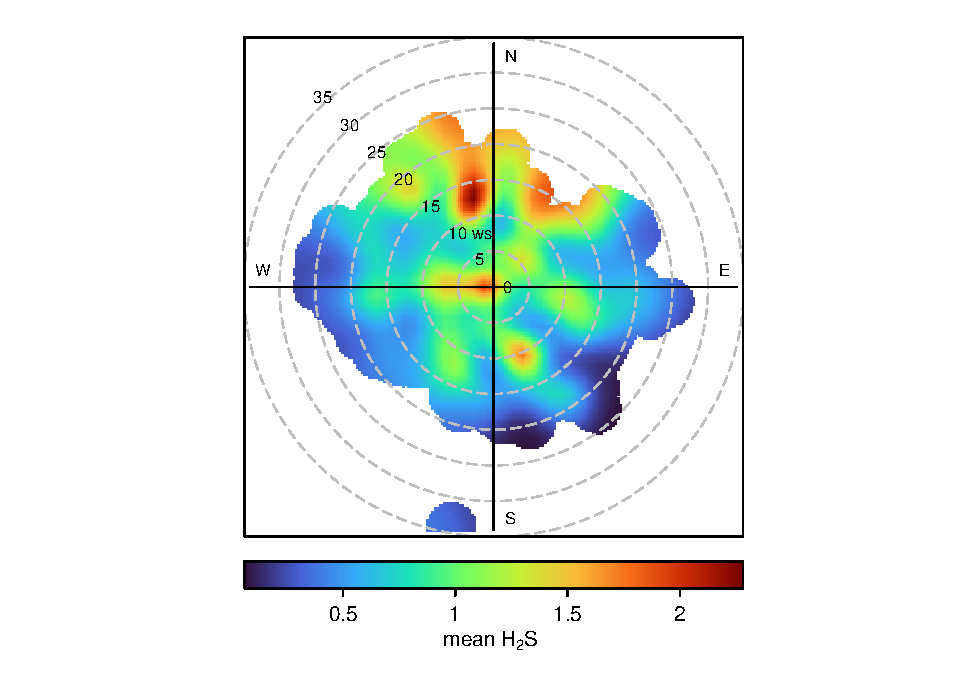
\includegraphics{data_merge_files/figure-latex/unnamed-chunk-8-1.pdf}
The line with the largest deviation/peak corresponds to the 213th\&Chico
monitor, in 2021-10

\begin{Shaded}
\begin{Highlighting}[]
\FunctionTok{library}\NormalTok{(openair)}
\end{Highlighting}
\end{Shaded}

\begin{verbatim}
## Warning: package 'openair' was built under R version 4.2.3
\end{verbatim}

\begin{Shaded}
\begin{Highlighting}[]
\NormalTok{full\_data }\SpecialCharTok{\%\textgreater{}\%}
  \FunctionTok{polarPlot}\NormalTok{(}\AttributeTok{pollutant =} \StringTok{"H2S"}\NormalTok{, }\AttributeTok{col =} \StringTok{"turbo"}\NormalTok{, }
            \AttributeTok{key.position =} \StringTok{"bottom"}\NormalTok{,}
            \AttributeTok{key.header =} \StringTok{"mean H2S"}\NormalTok{, }
            \AttributeTok{key.footer =} \ConstantTok{NULL}\NormalTok{)}
\end{Highlighting}
\end{Shaded}

\includegraphics{data_merge_files/figure-latex/unnamed-chunk-9-1.pdf}

\begin{Shaded}
\begin{Highlighting}[]
\NormalTok{full\_data }\OtherTok{\textless{}{-}}\NormalTok{ full\_data }\SpecialCharTok{\%\textgreater{}\%}
  \FunctionTok{mutate}\NormalTok{(}\AttributeTok{wd\_sec =} \FunctionTok{case\_when}\NormalTok{(}\DecValTok{0} \SpecialCharTok{\textless{}=}\NormalTok{ wd }\SpecialCharTok{\&}\NormalTok{ wd }\SpecialCharTok{\textless{}} \DecValTok{90} \SpecialCharTok{\textasciitilde{}} \StringTok{\textquotesingle{}Q1\textquotesingle{}}\NormalTok{,}
                            \DecValTok{90} \SpecialCharTok{\textless{}=}\NormalTok{ wd }\SpecialCharTok{\&}\NormalTok{ wd }\SpecialCharTok{\textless{}} \DecValTok{180} \SpecialCharTok{\textasciitilde{}} \StringTok{\textquotesingle{}Q2\textquotesingle{}}\NormalTok{,}
                            \DecValTok{180} \SpecialCharTok{\textless{}=}\NormalTok{ wd }\SpecialCharTok{\&}\NormalTok{ wd }\SpecialCharTok{\textless{}} \DecValTok{270} \SpecialCharTok{\textasciitilde{}} \StringTok{\textquotesingle{}Q3\textquotesingle{}}\NormalTok{,}
                            \DecValTok{270} \SpecialCharTok{\textless{}=}\NormalTok{ wd }\SpecialCharTok{\&}\NormalTok{ wd }\SpecialCharTok{\textless{}=} \DecValTok{360} \SpecialCharTok{\textasciitilde{}} \StringTok{\textquotesingle{}Q4\textquotesingle{}}\NormalTok{))}
\end{Highlighting}
\end{Shaded}

\begin{Shaded}
\begin{Highlighting}[]
\NormalTok{h2s\_model\_a }\OtherTok{\textless{}{-}} \FunctionTok{gam}\NormalTok{(H2S}\SpecialCharTok{\textasciitilde{}}\FunctionTok{s}\NormalTok{(}\FunctionTok{as.numeric}\NormalTok{(month),}\AttributeTok{bs=}\StringTok{\textquotesingle{}cc\textquotesingle{}}\NormalTok{)}\SpecialCharTok{+}\NormalTok{year}\SpecialCharTok{+}\NormalTok{wd\_sec}\SpecialCharTok{+}\NormalTok{ws}\SpecialCharTok{+}\NormalTok{MinDist}\SpecialCharTok{+}\NormalTok{Refinery, }\AttributeTok{data =}\NormalTok{ full\_data)}
\FunctionTok{summary}\NormalTok{(h2s\_model\_a)}
\end{Highlighting}
\end{Shaded}

\begin{verbatim}
## 
## Family: gaussian 
## Link function: identity 
## 
## Formula:
## H2S ~ s(as.numeric(month), bs = "cc") + year + wd_sec + ws + 
##     MinDist + Refinery
## 
## Parametric coefficients:
##                                     Estimate Std. Error t value Pr(>|t|)    
## (Intercept)                        2.625e-02  1.088e+00   0.024 0.980745    
## year2021                           2.902e-01  1.082e+00   0.268 0.788611    
## year2022                          -7.502e-01  1.083e+00  -0.693 0.488278    
## wd_secQ2                           9.199e-02  4.755e-02   1.935 0.053034 .  
## wd_secQ3                           8.023e-01  5.171e-02  15.515  < 2e-16 ***
## wd_secQ4                           4.519e-01  4.416e-02  10.232  < 2e-16 ***
## ws                                -9.079e-02  5.943e-03 -15.276  < 2e-16 ***
## MinDist                            3.945e-04  4.143e-05   9.522  < 2e-16 ***
## RefineryMarathon (Carson)          2.790e+00  6.251e-02  44.627  < 2e-16 ***
## RefineryMarathon (Wilmington)      1.220e+00  7.426e-02  16.431  < 2e-16 ***
## RefineryPhillips 66 (Wilimington) -2.243e-01  6.709e-02  -3.343 0.000828 ***
## RefineryPhillips 66 (Wilmington)   7.434e-01  6.600e-02  11.264  < 2e-16 ***
## RefineryTorrance Refinery         -3.084e-02  6.496e-02  -0.475 0.634929    
## RefineryValero Refinery            7.004e-01  6.374e-02  10.988  < 2e-16 ***
## ---
## Signif. codes:  0 '***' 0.001 '**' 0.01 '*' 0.05 '.' 0.1 ' ' 1
## 
## Approximate significance of smooth terms:
##                        edf Ref.df     F p-value    
## s(as.numeric(month)) 7.996      8 888.3  <2e-16 ***
## ---
## Signif. codes:  0 '***' 0.001 '**' 0.01 '*' 0.05 '.' 0.1 ' ' 1
## 
## R-sq.(adj) =  0.00853   Deviance explained = 0.854%
## GCV = 336.51  Scale est. = 336.51    n = 1730935
\end{verbatim}

\begin{Shaded}
\begin{Highlighting}[]
\FunctionTok{plot}\NormalTok{(h2s\_model\_a)}
\end{Highlighting}
\end{Shaded}

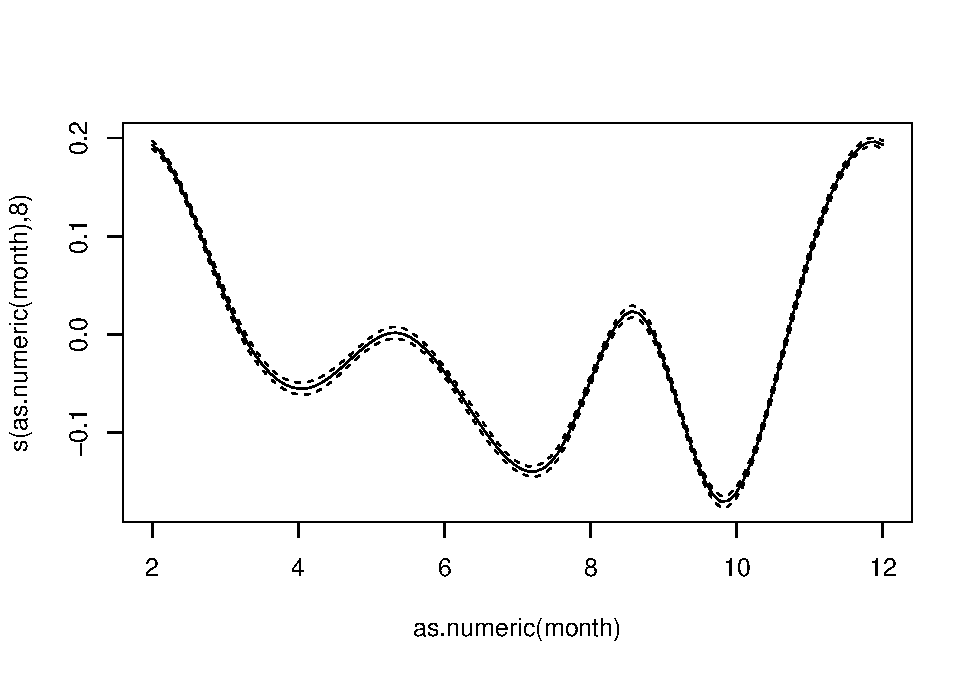
\includegraphics{data_merge_files/figure-latex/unnamed-chunk-11-1.pdf}

\begin{Shaded}
\begin{Highlighting}[]
\NormalTok{h2s\_dm\_model\_a }\OtherTok{\textless{}{-}} \FunctionTok{gam}\NormalTok{(H2S\_daily\_max}\SpecialCharTok{\textasciitilde{}}\FunctionTok{s}\NormalTok{(}\FunctionTok{as.numeric}\NormalTok{(month),}\AttributeTok{bs=}\StringTok{\textquotesingle{}cc\textquotesingle{}}\NormalTok{)}\SpecialCharTok{+}\NormalTok{year}\SpecialCharTok{+}\NormalTok{wd\_sec}\SpecialCharTok{+}\NormalTok{ws}\SpecialCharTok{+}\NormalTok{MinDist}\SpecialCharTok{+}\NormalTok{Refinery, }\AttributeTok{data =}\NormalTok{ full\_data)}
\FunctionTok{summary}\NormalTok{(h2s\_dm\_model\_a)}
\end{Highlighting}
\end{Shaded}

\begin{verbatim}
## 
## Family: gaussian 
## Link function: identity 
## 
## Formula:
## H2S_daily_max ~ s(as.numeric(month), bs = "cc") + year + wd_sec + 
##     ws + MinDist + Refinery
## 
## Parametric coefficients:
##                                     Estimate Std. Error t value Pr(>|t|)    
## (Intercept)                       -3.1472096  5.6784183  -0.554  0.57941    
## year2021                           1.1757710  5.6508473   0.208  0.83517    
## year2022                          -8.5505227  5.6514736  -1.513  0.13029    
## wd_secQ2                          -1.3227001  0.2444871  -5.410 6.30e-08 ***
## wd_secQ3                           3.4321149  0.2663043  12.888  < 2e-16 ***
## wd_secQ4                          -0.2189142  0.2274318  -0.963  0.33577    
## ws                                 0.0951378  0.0305405   3.115  0.00184 ** 
## MinDist                            0.0036415  0.0002139  17.025  < 2e-16 ***
## RefineryMarathon (Carson)         23.8627721  0.3216987  74.177  < 2e-16 ***
## RefineryMarathon (Wilmington)      7.4851108  0.3828418  19.551  < 2e-16 ***
## RefineryPhillips 66 (Wilimington)  1.9341546  0.3460242   5.590 2.28e-08 ***
## RefineryPhillips 66 (Wilmington)   6.3424509  0.3404535  18.629  < 2e-16 ***
## RefineryTorrance Refinery         -0.1880638  0.3347870  -0.562  0.57429    
## RefineryValero Refinery            6.8312347  0.3287783  20.778  < 2e-16 ***
## ---
## Signif. codes:  0 '***' 0.001 '**' 0.01 '*' 0.05 '.' 0.1 ' ' 1
## 
## Approximate significance of smooth terms:
##                        edf Ref.df    F p-value    
## s(as.numeric(month)) 7.998      8 2767  <2e-16 ***
## ---
## Signif. codes:  0 '***' 0.001 '**' 0.01 '*' 0.05 '.' 0.1 ' ' 1
## 
## R-sq.(adj) =  0.0231   Deviance explained = 2.31%
## GCV = 9172.2  Scale est. = 9172.1    n = 1777112
\end{verbatim}

\begin{Shaded}
\begin{Highlighting}[]
\FunctionTok{plot}\NormalTok{(h2s\_dm\_model\_a)}
\end{Highlighting}
\end{Shaded}

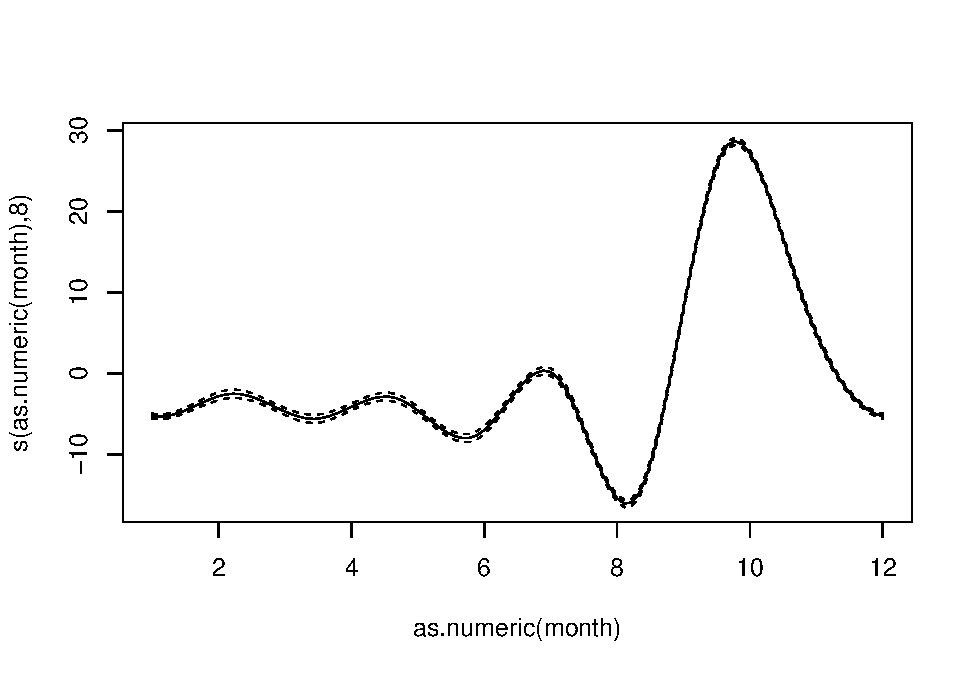
\includegraphics{data_merge_files/figure-latex/unnamed-chunk-12-1.pdf}

\begin{Shaded}
\begin{Highlighting}[]
\NormalTok{h2s\_ma\_model\_a }\OtherTok{\textless{}{-}} \FunctionTok{gam}\NormalTok{(H2S\_monthly\_average}\SpecialCharTok{\textasciitilde{}}\FunctionTok{s}\NormalTok{(}\FunctionTok{as.numeric}\NormalTok{(month),}\AttributeTok{bs=}\StringTok{\textquotesingle{}cc\textquotesingle{}}\NormalTok{)}\SpecialCharTok{+}\NormalTok{year}\SpecialCharTok{+}\NormalTok{wd\_sec}\SpecialCharTok{+}\NormalTok{ws}\SpecialCharTok{+}\NormalTok{MinDist}\SpecialCharTok{+}\NormalTok{Refinery, }\AttributeTok{data =}\NormalTok{ full\_data)}
\FunctionTok{summary}\NormalTok{(h2s\_ma\_model\_a)}
\end{Highlighting}
\end{Shaded}

\begin{verbatim}
## 
## Family: gaussian 
## Link function: identity 
## 
## Formula:
## H2S_monthly_average ~ s(as.numeric(month), bs = "cc") + year + 
##     wd_sec + ws + MinDist + Refinery
## 
## Parametric coefficients:
##                                     Estimate Std. Error t value Pr(>|t|)    
## (Intercept)                       -3.3920410  4.6395309  -0.731 0.464708    
## year2021                           0.9294228  4.6172234   0.201 0.840468    
## year2022                          -8.3528293  4.6177046  -1.809 0.070471 .  
## wd_secQ2                          -0.7166384  0.1981239  -3.617 0.000298 ***
## wd_secQ3                           2.8993293  0.2156818  13.443  < 2e-16 ***
## wd_secQ4                          -0.6605935  0.1845941  -3.579 0.000345 ***
## ws                                 0.1685881  0.0246061   6.851 7.31e-12 ***
## MinDist                            0.0035418  0.0001742  20.326  < 2e-16 ***
## RefineryMarathon (Carson)         22.1782910  0.2598275  85.358  < 2e-16 ***
## RefineryMarathon (Wilmington)      7.5832204  0.3114075  24.351  < 2e-16 ***
## RefineryPhillips 66 (Wilimington)  2.7139259  0.2813000   9.648  < 2e-16 ***
## RefineryPhillips 66 (Wilmington)   6.5865003  0.2770396  23.775  < 2e-16 ***
## RefineryTorrance Refinery          0.5419062  0.2681437   2.021 0.043285 *  
## RefineryValero Refinery            7.2127287  0.2668523  27.029  < 2e-16 ***
## ---
## Signif. codes:  0 '***' 0.001 '**' 0.01 '*' 0.05 '.' 0.1 ' ' 1
## 
## Approximate significance of smooth terms:
##                        edf Ref.df    F p-value    
## s(as.numeric(month)) 7.999      8 4021  <2e-16 ***
## ---
## Signif. codes:  0 '***' 0.001 '**' 0.01 '*' 0.05 '.' 0.1 ' ' 1
## 
## R-sq.(adj) =  0.0309   Deviance explained = 3.09%
## GCV = 6123.7  Scale est. = 6123.7    n = 1814982
\end{verbatim}

\begin{Shaded}
\begin{Highlighting}[]
\FunctionTok{plot}\NormalTok{(h2s\_ma\_model\_a)}
\end{Highlighting}
\end{Shaded}

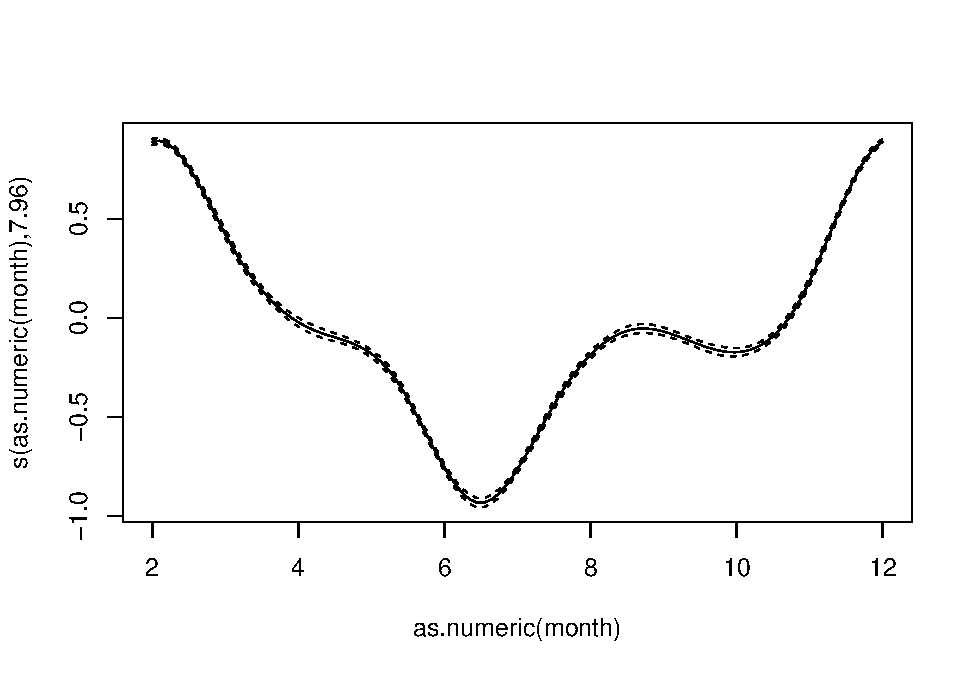
\includegraphics{data_merge_files/figure-latex/unnamed-chunk-13-1.pdf}

\begin{Shaded}
\begin{Highlighting}[]
\FunctionTok{saveRDS}\NormalTok{(full\_data, }\StringTok{\textquotesingle{}data/full\_data.rds\textquotesingle{}}\NormalTok{)}
\end{Highlighting}
\end{Shaded}


\end{document}
